\subsection{Разработка программной части комплекса}

\begin{frame}{NodeJS}
  Использованные пакеты Node.JS:

  \begin{enumerate}
    \item rpi-ws281x-native --- управление адресной светодиодной лентой;
    \item child\_process --- запуск дочерних процессов.
  \end{enumerate}
\end{frame}

\section{Программно-аппаратный комплекс}

\begin{frame}{Готовый программно-аппаратный комплекс}
  Собранный программно-аппаратный комплекс

  \begin{figure}[H]
    \centering
    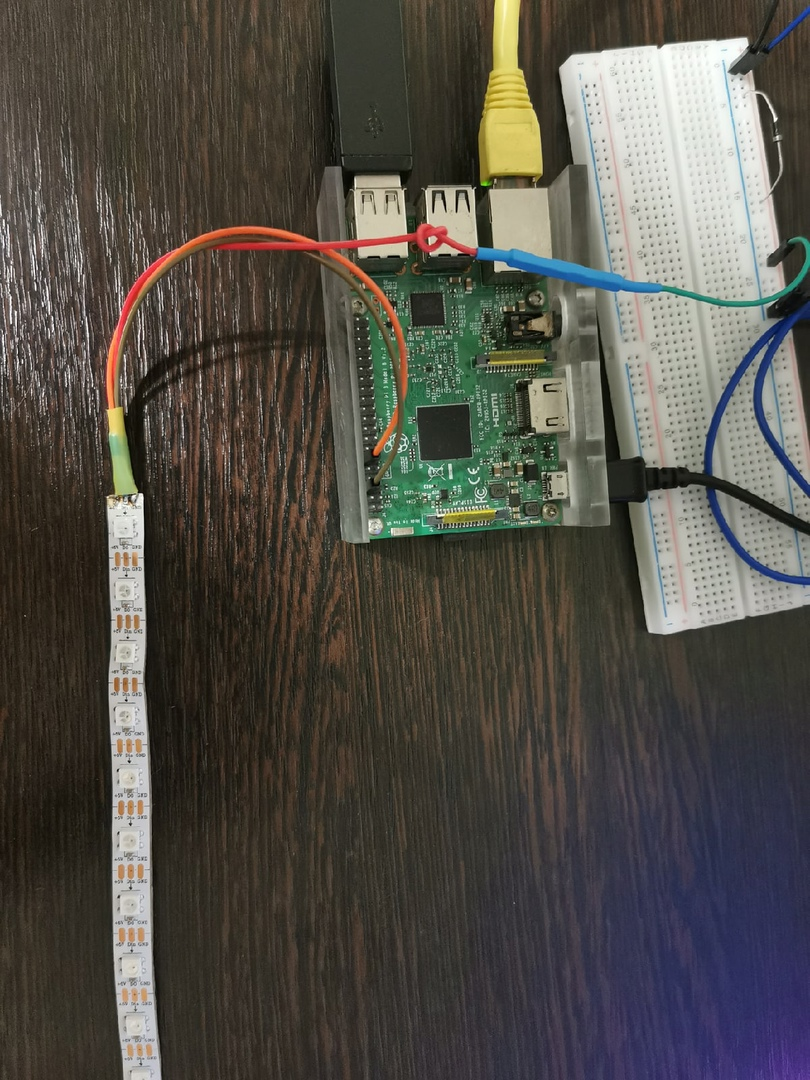
\includegraphics[angle=90, width=0.65\textwidth]{assets/images/Полная схема.jpg}
  \end{figure}
\end{frame}

\begin{frame}{Готовый программно-аппаратный комплекс}
  Пример работы

  \begin{figure}[H]
    \centering
    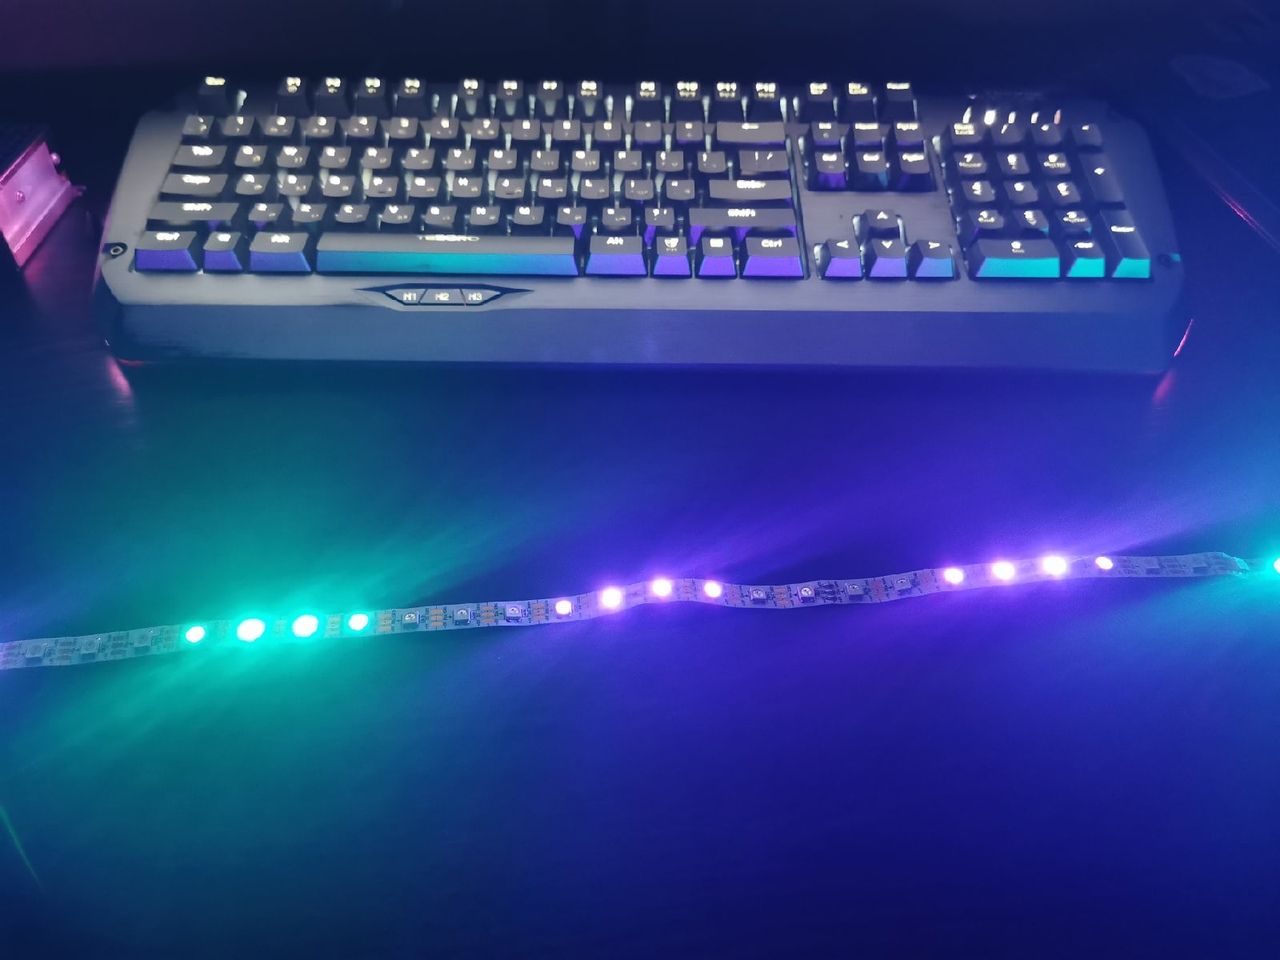
\includegraphics[height=0.75\textheight]{assets/images/ws2812__in_work.jpg}
  \end{figure}
\end{frame}
